% =====================================================================
% Modelagem do grafo: justificativa e diagrama de classes --- Brunno (Frente 1)
% =====================================================================
\section{Modelagem do grafo}\label{sec:modelagem}

\subsection{O que é nó e o que é aresta}

Cada rede vira um grafo $G = (V, E)$ não direcionado e simples (sem arestas repetidas),
com $n = |V|$ nós e $m = |E|$ arestas. Na Twitch PT, cada nó é um streamer e cada aresta é
uma amizade mútua, sem peso. No ego-Facebook, os nós são usuários e as arestas, amizades.
No Karate Club, os nós são membros do clube e as arestas, interações fora das aulas. Na
Network of Thrones, os nós são personagens e cada aresta tem peso $w(e)$ igual ao número de
interações entre os dois no livro. Grafos sem peso usam $w(e) = 1$.

\subsection{Por que lista de adjacência}

As redes sociais são esparsas: cada pessoa se liga a uma fração pequena das outras. Na
Twitch PT, a densidade é $2m/(n(n-1)) \approx 0{,}017$, ou seja, só 1,7\% dos pares possíveis
são amizades. Uma matriz de adjacência guardaria $n^2 = 3{,}66$ milhões de células, 98\% delas
com zero, e gastaria $O(n^2)$ de memória. A lista de adjacência guarda só as arestas que
existem, em $O(n + m)$, e percorre os vizinhos de um nó $v$ em $O(\text{grau}(v))$. Por isso
a busca em largura custa $\Theta(n + m)$ com lista e $\Theta(n^2)$ com
matriz~\cite{cormen2022,sedgewick2011}, e quase todos os algoritmos do trabalho dependem
desse percurso.

\subsection{Por que um dicionário de dicionários}

A classe \codigo{Grafo} guarda a lista de adjacência como um dicionário de dicionários:
\codigo{\_adj[v][w]} é o peso da aresta entre $v$ e $w$. Três motivos levaram a essa escolha:
\begin{itemize}
  \item testar se uma aresta existe custa $O(1)$ em média, enquanto um dicionário de listas
        exigiria percorrer os vizinhos, em $O(\text{grau}(v))$~\cite{pythoncomplexidade};
  \item o peso fica junto do vizinho, o que atende a Network of Thrones e o Louvain, que cria
        arestas com peso ao agrupar comunidades~\cite{blondel2008};
  \item os nós podem ser de qualquer tipo imutável: números na Twitch e nomes na Network of Thrones.
\end{itemize}
O NetworkX, que só usaremos para comparar desempenho, adota a mesma estrutura pelos mesmos
motivos~\cite{hagberg2008}. A Tabela~\ref{tab:complexidade} resume o custo das operações.

\begin{table}[htbp]
\centering
\caption{Custo das operações da classe \codigo{Grafo} ($O(1)$ em média, pelo uso de dicionários).}
\label{tab:complexidade}
\small
\begin{tabular}{@{}l l@{}}
\toprule
Operação & Tempo \\
\midrule
Inserir nó, inserir ou remover aresta & $O(1)$ \\
Testar aresta, ler peso, grau & $O(1)$ \\
Percorrer os vizinhos de $v$ & $O(\text{grau}(v))$ \\
Listar todas as arestas & $O(n + m)$ \\
Número de nós e de arestas & $O(1)$ \\
Memória total & $O(n + m)$ \\
\bottomrule
\end{tabular}
\end{table}

\subsection{Outras decisões}

\begin{itemize}
  \item \textbf{Grafos direcionados:} a classe também os aceita. Nesse caso, guarda à parte os
        predecessores de cada nó (\codigo{\_pred}), para calcular o grau de entrada e o
        PageRank~\cite{brin1998} sem percorrer o grafo inteiro. No não direcionado,
        \codigo{\_pred} é o próprio \codigo{\_adj}, sem cópia.
  \item \textbf{Laços:} a classe aceita a aresta $(v, v)$, que o Louvain cria ao agrupar
        comunidades, e a conta duas vezes no grau, para a soma dos graus ser sempre $2m$.
        Os leitores das bases descartam laços, que nelas são ruído.
  \item \textbf{Contador de arestas:} o número de arestas $m$ é mantido a cada inserção e
        remoção, e sai em $O(1)$; ele aparece na densidade, no grau médio e na modularidade.
  \item \textbf{Reindexação:} nos algoritmos pesados (betweenness de Brandes e PageRank), os nós
        são renumerados de $0$ a $n-1$ e a adjacência vira uma lista de listas, que tem custo
        constante menor que o dicionário.
\end{itemize}

\subsection{Diagramas de classes e de pacotes}

A Figura~\ref{fig:classes} detalha o núcleo: a classe \codigo{Grafo} e o
\codigo{IndexadorDeNos}, que renumera os nós de $0$ a $n-1$ para os algoritmos pesados.
A Figura~\ref{fig:pacotes} mostra como o resto do código se organiza em volta dele. Os demais
pacotes são módulos de funções que recebem um \codigo{Grafo}, não o alteram e devolvem um
resultado por nó (\codigo{dict[nó, valor]}), um contrato comum a todas as frentes. Os leitores
e os geradores criam grafos; a interface só chama as funções e mostra os resultados. O NetworkX
aparece apenas em \codigo{desempenho/}, para a comparação permitida pelo enunciado.

\begin{figure}[htbp]
\centering
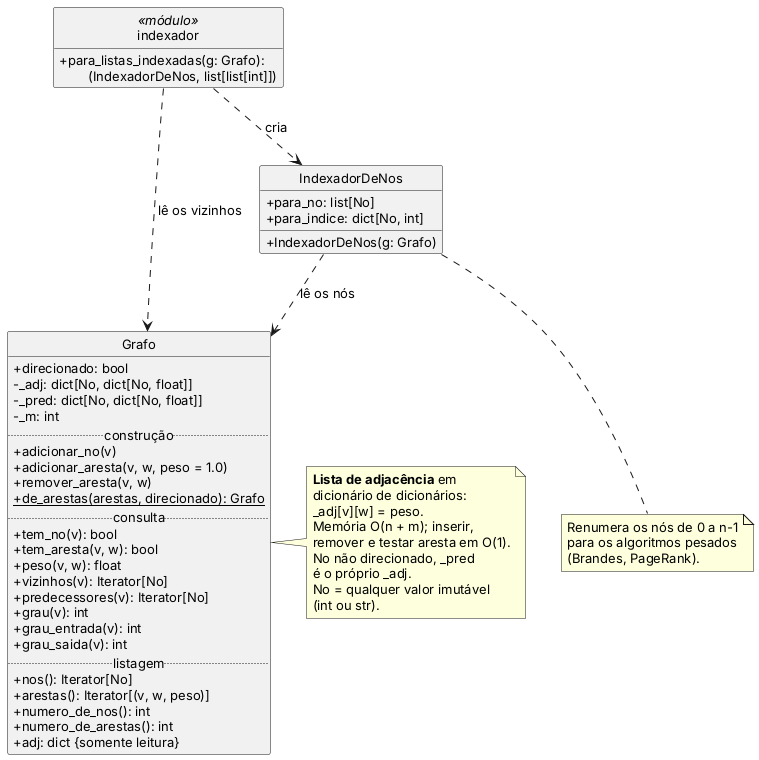
\includegraphics[width=.9\textwidth]{classes.png}
\caption{Diagrama de classes do núcleo (\codigo{redes/nucleo}).}
\label{fig:classes}
\end{figure}

\begin{figure}[htbp]
\centering
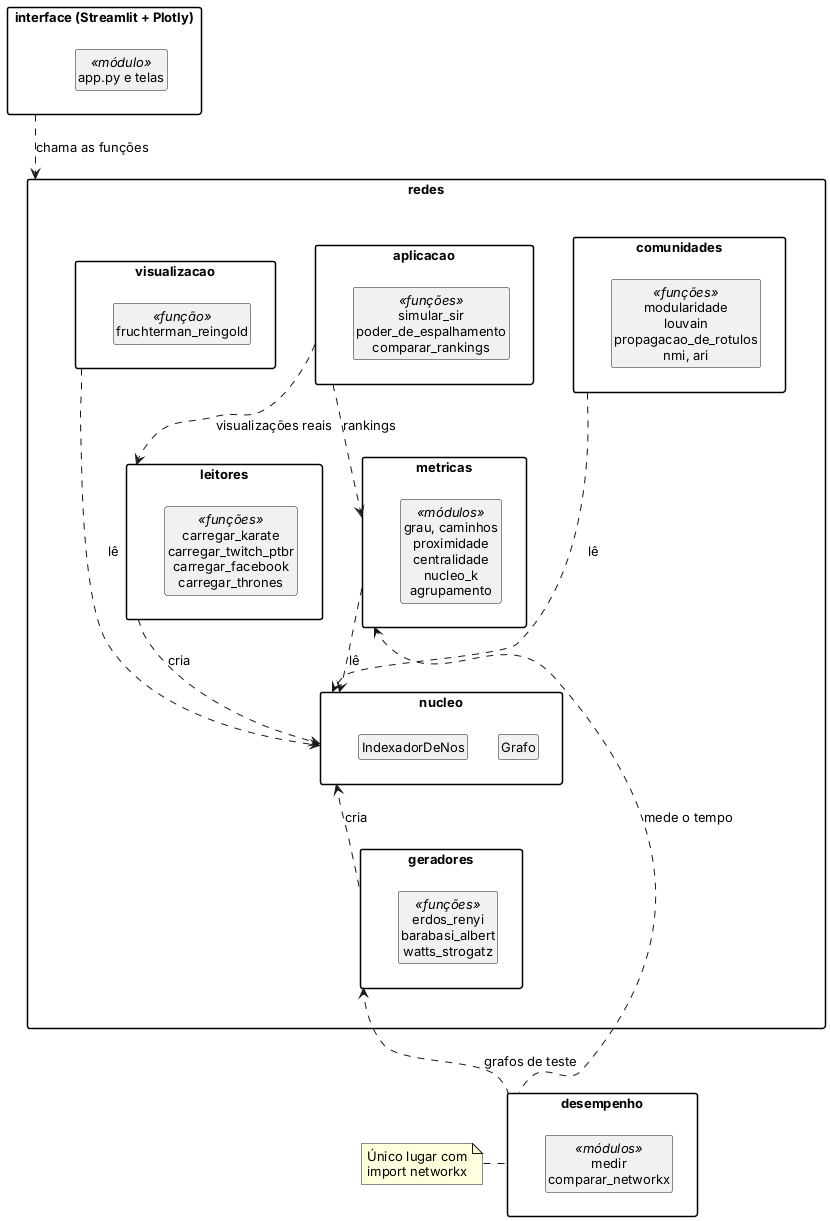
\includegraphics[width=.85\textwidth]{pacotes.png}
\caption{Diagrama de pacotes da ferramenta. As setas tracejadas indicam dependência: quem
  aponta usa o pacote apontado.}
\label{fig:pacotes}
\end{figure}
